%%%%%%%%%%%%%%%%%%%%%%%%%%%%% -*- Mode: Latex -*- %%%%%%%%%%%%%%%%%%%%%%%%%%%%
%% 05-01-system.tex -- Thesis Proposal - PRI
%% Author          : Aaron A. Kagawa
%% Created On      : Mon Sep 23 11:52:28 2004
%% Last Modified By: Aaron Kagawa
%% Last Modified On: Tue Jul  5 20:16:17 2005
%% RCS: $Id$
%%%%%%%%%%%%%%%%%%%%%%%%%%%%%%%%%%%%%%%%%%%%%%%%%%%%%%%%%%%%%%%%%%%%%%%%%%%%%%
%%   Copyright (C) 2004 Aaron A. Kagawa
%%%%%%%%%%%%%%%%%%%%%%%%%%%%%%%%%%%%%%%%%%%%%%%%%%%%%%%%%%%%%%%%%%%%%%%%%%%%%%%

\chapter{Implementing PRI with Hackystat}
\label{chapter:system}
To successfully use Priority Ranked Inspection, the determination of MINI
and LINI must be obtainable for a very low cost. In other words, if the
ranking function takes three months, or even 20 hours of management time to
generate, then a software project may no longer need those specific
recommendations. Therefore, this determination must be obtained in
real-time and without introducing new costs to the inspection process.

One way of obtaining PRI rankings in real-time and without developer
overhead is through the use of the Hackystat system \cite{Johnson05}.
Hackystat is a framework for collecting and analyzing software product and
development process metrics in real-time \footnote{For more information
  about the Hackystat system see Chapter \ref{chapter:hackystat}.}. For
this research, I have created an extension to Hackystat called the
Hackystat Priority Ranked Inspection Extension (hackyPRI for short). This
extension provides a real-time PRI ranking. Figure
\ref{fig:PriRankingAnalysis} demonstrates the use of the PRI ranking
function by ranking a software project's workspaces.

This chapter provides a detailed description of the Hackystat PRI
(hackyPRI) extension. In Section \ref{section:limitations}, I identify the
limitations of implementing the PRI process with Hackystat. Section
\ref{section:prirankingfunction} provides a general introduction to the PRI
ranking function. Section \ref{section:userinterface} provides a user level
description of how to use the hackyPRI extension. Section
\ref{section:foursteps} discusses how hackyPRI supports the four steps of
the Priority Ranked Inspection process. Section
\ref{section:designAndImplementation} provides a developer level
explanation of the extension's design and implementation. Section
\ref{section:future} discusses the future enhancements that could be added
to hackyPRI. Section \ref{section:contributions} provides a list of
contributions that I have added to the Hackystat system as a result of my
implementation of hackyPRI. Finally, Section \ref{section:using} provides
some information for other organizations to install and use hackyPRI.


\begin{figure*}[htbp]
  \centering
  \includegraphics[height=1.00\textheight]{figs/2005-04-25-cropped-hidden.eps}
  \caption[PRI Ranking analysis]{The PRI analysis. Workspaces are listed
    with its respective PRI ranking and measures.}
  \label{fig:PriRankingAnalysis}
\end{figure*}



\section{Limitations of Implementing PRI with Hackystat}
\label{section:limitations}
Certainly, utilizing the real-time and low-developer-overhead collection
and analysis features of Hackystat is not perfect for every organization.
There are many adoption barriers that come with a PRI process implemented
with Hackystat. For example, the barriers could include the initial cost of
setting up and using Hackystat to collect process and product measures, the
configuration of the ranking function, the devotion required to ensure that
Hackystat provides accurate information, privacy issues associated with
collecting information on developers, and possibly many more.  In addition,
although it is yet to be studied, I hypothesize that PRI will not be
instantaneously beneficial to an organization. In other words, if an
organization installs, configures, and uses hackyPRI for only one week,
then I believe the rankings will not be as beneficial as compared to
another organization that has collected 3 years of Hackystat data.

I have designed the general theory of the Priority Ranked Inspection
process to be independent of any specific means of collection, analysis,
and ranking.  However, I have chosen to use Hackystat to implement PRI in
this research, because the organization that I am studying has already
faced and found solutions for the barriers listed above. 



\section{PRI Ranking Function}
\label{section:prirankingfunction}
The PRI ranking function is the most important and most complicated
component of hackyPRI. There are two fundamental components in the PRI
ranking function that must be understood by both users and developers of
hackyPRI. They are the PRI measures and the PRI indicators. The following
sections introduce these concepts.

\subsection{PRI Measures}
PRI measures represent the product and process measures that are the basis
for determining whether a document is a MINI or a LINI. In addition, they
are used to help generate the rankings of documents and help explain the
rankings by displaying the measure values. To better illustrate this, see
Figure \ref{fig:PriRankingAnalysis}. This figure presents a PRI ranking
obtainable from hackyPRI. The figure contains a listing of the project's
workspaces and its associated values collected from the PRI measures. In
theory, PRI measures can be associated with any granularity level of a
software artifact; for example, documents, packages, workspaces, and
modules. Currently, I have only implemented a set of PRI measures that work
for workspaces within a project.

\subsubsection{Collection of PRI Measures}
PRI measures provide the values of product and process measures associated
with each document. In the general theory of the Priority Ranked Inspection
process, PRI measures can be collected by any means. In hackyPRI, the
Hackystat system is used to automate the collection of the PRI measures. In
Hackystat, product and process measures are represented by three
components. They are the Sensor Data Type, Sensor, and DailyProjectData
components. A Sensor Data Type defines the attributes associated with a
measure. A Sensor is used to collect the measures and send that information
to a Hackystat server. The DailyProjectData provides a project-level
representation of the low-level data that was collected by the Sensors.
hackyPRI requires the use of these three components; therefore one must
have the necessary Hackystat knowledge to successfully implement a PRI
measure. In addition to the three Hackystat components, hackyPRI implements
another component that represents a PRI measure, which is used within the
PRI ranking. Section \ref{section:designAndImplementation} explains the
implementation of PRI measures in detail.

\subsubsection{Aggregate and Snapshot PRI Measures}
There are two different types of PRI measures. They are Aggregate and
Snapshot measures. An Aggregate PRI measure is the result of the summation
of calculated values obtained from processing one or more days of Hackystat
Sensor Data. For example, the Active Time PRI measure is an Aggregate
measure because it adds the values of active time over a specified time
period. If a developer has generated 1.2, 1.0, and 2.0 hours of active time
on three successive days, the Aggregate Active Time measure would return
4.2 hours. Snapshot measures are not aggregated. Instead, they represent
the most recent value of a measure from one or more days. For example, the
LOC (lines of code) measure does not make sense as an Aggregate measure.
If the system size was 1000, 1100, and 1200 on three successive days, then
the aggregate of those numbers (3300) is not useful. Therefore, LOC is a
Snapshot PRI measure, and in this example 1200 is returned. In hackyPRI,
Aggregate and Snapshot measures must be implemented differently. Therefore,
the decision of the type of PRI measure (either Aggregate or Snapshot) must
be made carefully.

\subsection{PRI Indicators}
\label{subsection:priIndicators}
PRI indicators use one to many PRI measures to provide a ranking for each
document. PRI indicators provide indications of whether documents are MINI
or LINI. For example, the Testing PRI indicator provides indications on
whether a document has adequate testing. This indicator accesses the Unit
Test, Coverage, and Test Code Active Time PRI measures to evaluate the
level of testing for the document.

PRI indicators have the following characteristics. First, PRI indicators
determine whether a document is a MINI or a LINI. Second, each PRI
indicator can use the data from one or many PRI measures. Third, each PRI
indicator returns an integer value between 0 and 100. Fourth, different
weights can be assigned to different PRI indicators.

The calibration of the PRI indicators' ranking and weights is a very
important step when using hackyPRI. Each individual PRI indicator can and
should be calibrated differently to provide a PRI ranking that best
represents a MINI and LINI determination for a specific project. The
calibration of a PRI indicator includes four steps.

\begin{enumerate}
\item \textbf{0 to 100 indicator ranking} - Once a PRI measure has gathered
  and calculated data from the product and process measures obtainable from
  Hackystat, its values are used within PRI indicators to return a ranking
  from 0 to 100. A zero ranking indicates the worst possible ranking and a
  hundred ranking indicates the best possible ranking. For example, in the
  Coverage (the percentage of code exercised by test cases) PRI indicator,
  one could imagine that 0 ranking would indicate 0 percent coverage and a
  100 ranking would be reserved for 100 percent coverage. To calculate a
  ranking, certain thresholds must be identified that are specific for each
  PRI indicator.  This is hard for some indicators and easy for others. In
  the Coverage PRI indicator, this is relatively straight forward, because
  the indicator relies on a single PRI measure and the coverage percentage
  is already on a 0-100 scale. On the other hand, the thresholds for the
  Testing PRI Indicator are less clear.  The Testing PRI Indicator uses
  three different measures, the PRI Unit Test measure, the PRI Coverage
  measure, and the PRI Active Time measure.  In addition, the values of
  these measures, when combined, do not fit nicely into a 0-100 scale.
  Currently, calculation of the indicator rankings is implemented with Java
  code within the hackyPRI system.
\item \textbf{Weights are assigned to each indicator} - It is possible that
  each PRI indicator affects the ranking differently. Therefore, each
  indicator can be given a different weight to reflect that difference. For
  example, an organization may find that coverage is the leading indicator
  of MINI documents and can weight coverage higher than any other PRI
  indicator.  Weights can range from 0 to any integer. If an indicator has
  a weighting of 0, then this indicator will be ``disabled'' from the
  ranking function.  These weighting are configurable through the hackyPRI
  user interface for each project within Hackystat and all indicators are
  defaulted to a weighting of 1 in the initial configuration of a Project
  PRI Ranking.
\item \textbf{Compute aggregate ranking for all indicators} - Once the
  independent ranking and weights are in place, the system will
  automatically compute an aggregate ranking per document. A very simple
  example is the following: a document has these indicator rankings \{92,
  100, 30, 15\} and these respective indicator weighting \{1, 1, 1, 2\}.
  The aggregate ranking of this document would be (92*1) + (100*1) + (30*1)
  + (15*2) = 252.
%% Not normalized, so not able to compare over time
\item \textbf{MINI and LINI declaration} - The final step of this process
  is the declaration of MINI and LINI for each document based on the
  aggregate ranking. Currently, I have not implemented the facilities to
  make a declaration of MINI and LINI, because this has proven to be more
  difficult than I first envisioned. I will leave this as a future
  implementation and research task. However, the current system does
  provide a 'relative' ranking: a workspace with a higher PRI ranking is
  ``more MINI'' than all workspaces with a lower PRI ranking. In addition,
  Hackystat projects generally have hundreds, if not thousands, of
  different workspaces, therefore a relative ranking is sufficient for this
  current research.
\end{enumerate}




\section{User Interface}
\label{section:userinterface}
This section contains a description of important hackyPRI user interface
components. It should be noted that, like most Hackystat user interface
components, the interface components associated with hackyPRI have not been
thoroughly tested for usability problems using traditional Human Computer
Interaction evaluation techniques. However, the developers of Hackystat
have informally reviewed the user interface.

Each description of the hackyPRI user interface components in this section
will be accompanied by a screenshot.

\clearpage
\subsection{PRI Analyses}
\begin{figure*}[htbp]
  \centering
  \includegraphics[width=1.00\textwidth]{figs/UserInterface/section-projectPriRanking.eps}
  \caption[PRI analyses]{Presents the analyses that are provided by the
    hackyPRI system.}
  \label{fig:section-projectPriRanking}
\end{figure*}
This screenshot shows the Hackystat analyses that the hackyPRI system
provides. The List Workspace analysis, the first Hackystat analysis in the
screenshot, allows users to validate the set of workspaces associated with
a specific project. Because, the PRI ranking provides rankings for
workspaces it is important to ensure that all workspaces within your
project are used in the PRI ranking. Therefore, it is very important that
all the project's workspaces, including child workspaces, are identified
by this analysis.

The Project PRI Module Ranking analysis, the second Hackystat analysis in
the screenshot, displays the PRI ranking for top-level workspaces, or
modules. This analysis ranks the modules by the average PRI rankings for
all workspaces within the modules. 

The Project PRI Ranking analysis, the third Hackystat analysis in the
screenshot, provides the PRI ranking for workspaces within the selected
Project. The execution of this analysis results in a table that ranks
workspaces within the project according to the PRI ranking function
described in Section \ref{subsection:priIndicators}. Before using this
analysis, you must configure the PRI ranking, see Section
\ref{subsection:configurationManagement}.



\clearpage
\subsection{PRI List Workspace Analysis}
\begin{figure*}[ht]
  \centering
  \includegraphics[width=1.00\textwidth]{figs/UserInterface/analysis-listWorkspace.eps}
  \caption[Execution of the List Workspace analysis]{Presents an example execution
    of the List Workspace analysis.} 
  \label{fig:analysis-listWorkspace}
\end{figure*}
This screenshot shows the result of the Hackystat List Workspace analysis.
This analysis allows users to validate the set of workspaces associated
with a specific project. Because, the PRI ranking provides rankings for
workspaces it is important to ensure that all workspaces within your
project are identified.

This screenshot provides a table of all workspaces within a project. In
this particular execution, there are 1564 workspaces associated with the
hacky2004-all Project. These are the workspaces that will be ranked by the
PRI Ranking analysis. However, due to configurations that specify the
programming language used in the hacky2004-all project, workspaces without
Java software code are ignored from the ranking. Therefore, most of the
1,564 workspaces will not be ranked.

\clearpage
\subsection{Project PRI Configuration Management}
\label{subsection:configurationManagement}
\begin{figure*}[ht]
  \centering
  \includegraphics[width=1.00\textwidth]{figs/UserInterface/preference-config-kagawaa.eps}
  \caption[Project PRI Configuration Management preference page]{The
    Preference page that presents the Project PRI Configuration management.}
  \label{fig:preference-config-kagawaa}
\end{figure*}
This screenshot presents the Project PRI Configuration Management page. The
configuration management is accessible on the Hackystat preferences page,
shown in the screenshot in Figure \ref{fig:page-preferences}. All software
projects are different; therefore the purpose of the configuration
management page is to configure the PRI ranking function for a specific
project.

There are two different sets of configurations shown in this screenshot.
The first table shows the PRI configurations associated with Hackystat
Projects that you own. The second table shows PRI configurations associated
with projects that you are a member of. The configuration management only
allows users to create PRI configurations for the projects that they own.
For example, I must contact johnson@hawaii.edu, the Project Owner for
hacky2004-all, to create a PRI configuration for the hacky2004-all project.
Once a Project PRI configuration is created, then the Project Owner can
modify and delete the configuration.

%%\clearpage
%%\subsection{Project PRI Configuration Management}
%%\begin{figure*}[ht]
%%  \centering
%%  \includegraphics[width=1.00\textwidth]{figs/UserInterface/preference-config-johnson.eps}
%%  \caption[Project PRI Configuration Management preference page]{The
%%    Preference page that presents the Project PRI Configuration management.}
%%  \label{fig:preference-config-johnson}
%%\end{figure*}


\clearpage
\subsection{Create a Project PRI Configuration}
\label{subsection:createPriConfiguration}
\begin{figure*}[ht]
  \centering
  \includegraphics[width=1.00\textwidth]{figs/UserInterface/preference-createConfig-hacky2004all-johnson-full.eps}
  \caption[Create Project PRI Configuration]{The Create a PRI Configuration 
    page.}
  \label{fig:preference-createConfig-hacky2004-all-jonhson-full}
\end{figure*}
In the previous section, I explained that only a Project Owner has the
authority to create a PRI configuration. Therefore, in this example, I've
contacted the project owner and requested the creation of the PRI
configuration for the hacky2004-all Project. This screenshot presents the
Create Project PRI Configuration webpage. To create a configuration, we
must provide the following information:

\begin{enumerate}
\item \textbf{File Extension} - this setting allows the specification of
  the type of programming language that is used in the PRI Ranking for this
  Project.  Valid entries are file extensions that contain a ``.'' followed
  by any number of characters. For example, a valid entry could be
  ``.java'', ``.cpp'', ``.html'', or whatever programming language file
  extension is associated with your project. There are some problems
  associated with this setting. First, this setting does not support
  Projects that are implemented with more than one programming language.
  Second, the Hackystat product and process measures implemented within
  Hackystat best support the Java Programming language. Other programming
  languages, like C and C++, are supported but not to the extent of Java.
  Furthermore, I did not test the generation of PRI racking for other
  programming languages other than Java. Of course, the hackyPRI and
  Hackystat systems can be fairly easy to extend to fully support any
  programming language.  However, for this research I will leave these
  issues as a future enhancement.
\item \textbf{Ignored Workspace Pattern(s)} - this setting allows the
  specification of workspaces that should be ignored in the PRI ranking.
  Simply put, I have found that some workspaces in a Project do not need to
  be inspected. This can happen for a couple of reasons. First, some
  workspaces contain code that is no longer released. Second, some code,
  for example, automatically generated code, could be ignored. This is a
  debatable use of the ignored workspace pattern, but it is provided to the
  user as an option.
  
  In this screenshot, the ``hackyCourse'', ``hackyPrjSize'',
  ``hackyCocomo'', ``hackySQI'', and ``hackyJPLBuild'' are parent
  workspaces that should be ignored. The configuration will also ignore any
  child workspace under those parent workspaces. The ``selector'' ignored
  workspace pattern, specifies that any workspaces that contains the string
  ``selector'' shall also be ignored. For the hacky2004-all project,
  selector code is an anomaly that generally does not need to be inspected.
\item \textbf{Indicator Weighting} - this setting allows the specification
  of the weights associated with the PRI indicators. By default, all PRI
  indicator weights are set to 1. Any positive integer, including zero, are
  valid weights. The indicator weights are used to calibrate the individual
  PRI indicator rankings, Section \ref{subsection:priIndicators} explains
  this in detail. If a weight is set to zero, then the PRI indicator will
  not affect the PRI ranking. If an indicator's weight is set to 2, and all
  other weighting remain at 1, then the indicator will have twice the
  significance as the other indicators. Indicator weighting is useful to
  correctly configure the indicators' importance in the PRI ranking. For
  example, if Coverage is a leading factor in the PRI ranking, then it
  should be weighted higher than the other indicators.
\end{enumerate}


\clearpage
\subsection{Project PRI Configuration Management - After the Creation of a 
  PRI Configuration}
\begin{figure*}[ht]
  \centering
  \includegraphics[width=1.00\textwidth]{figs/UserInterface/preference-configAfterCreate-johnson.eps}
  \caption[Project PRI Configuration Management preference page]{The
    Preference page that presents the Project PRI Configuration management.}
  \label{fig:preference-configAfterCreate-johnson}
\end{figure*}
This screenshot presents the Project PRI configuration management webpage
after the creation of a PRI configuration. Provided in the webpage are the
details of the configurations that have been created. In addition, the
Project Owner can modify and delete the configuration.

%%\clearpage
%%\subsection{Project PRI Configuration Management}
%%\begin{figure*}[ht]
%%  \centering
%%  \includegraphics[width=1.00\textwidth]{figs/UserInterface/preference-configAfterCreate-kagawaa.eps}
%%  \caption[Project PRI Configuration Management preference page]{The
%%    Preference page that presents the Project PRI Configuration management.}
%%  \label{fig:preference-configAfterCreate-kagawaa}
%%\end{figure*}


\clearpage
\subsection{Project PRI Ranking Analysis}
\label{subsection:projectPriRanking}
\begin{figure*}[ht]
  \centering
  \includegraphics[width=1.00\textwidth]{figs/UserInterface/analysis-priRanking-sortByRanking-full-hidden.eps}
  \caption[Execution of the Project PRI Ranking analysis]{Presents an
    example execution of the Project PRI Ranking analysis.}  
  \label{fig:analysis-priRanking-full}
\end{figure*}
After a Project PRI configuration has been successfully created and
configured in the previous sections, then you can run the PRI Ranking
analysis. The analysis is obtainable on the analyses page (Figure
\ref{fig:page-analysis}) in the Project PRI Ranking section (Figure
\ref{fig:section-projectPriRanking}).

This screenshot presents the rankings of the hacky2004-all project. This
project contains the product and process measures that have been collect
during the development of the Hackystat system. I will be using this
Hackystat project to evaluate the hackyPRI system. 

Due to page width constraints, the screenshot does not show the values of
the numerous PRI measures and all the workspaces available. Normally, in
this table you will be able to view the workspace, the aggregate ranking,
and all the values of each of the PRI measures. This particular execution
of the analysis  ranks each workspace by its associated aggregate PRI
ranking. It sorts the highest ranked workspaces (LINI) to the top of the
table and the lowest ranked workspaces (MINI) to the bottom of the table.

%%\clearpage
\subsection{Project PRI Ranking Analysis Selectors}
\begin{figure*}[ht]
  \centering
  \includegraphics[width=1.00\textwidth]{figs/UserInterface/analysis-priRanking-command.eps}
  \caption[Project PRI Ranking analysis selectors]{Presents the
    selectors that are available in the Project PRI Ranking analysis.}
  \label{fig:analysis-priRanking-command}
\end{figure*}
This screenshot presents the user interface for the PRI Ranking analysis.
There are five different selectors that users can set to determine the PRI
Ranking that they would like to generate.

\begin{enumerate}
\item \textbf{Project PRI Configuration} - users should use this selector
  to select what PRI configuration they would like to be used in the PRI
  ranking. A PRI configuration has a one-to-one correspondence with
  Hackystat Projects, thus when you select a PRI configuration you are also
  selecting what Project data to use in the PRI ranking. PRI configurations
  must be created using the PRI Configuration Management preference
  interface before a PRI ranking can be generated (See Section
  \ref{subsection:configurationManagement} and
  \ref{subsection:createPriConfiguration}).
\item \textbf{Package Filter} - users should use this selector to show
  workspaces that contain a value of the string they enter into the
  textbox. For example, if a user wants to generate the PRI ranking only
  for the hackyKernel module, then they should enter in ``hackyKernel''
  into the Package Filter selector.  Section
  \ref{subsection:projectPriRanking-hackyKernel} contains a screenshot of
  an example use of this selector. In addition, if a user wants to rank
  only analysis code, then the user can enter in ``analysis'' and all
  workspaces that contain that value will be ranked.
\item \textbf{Refresh Calculation?} - users should use this selector to
  either re-generate the PRI ranking or use the last PRI ranking stored in
  the system. This is an unusual and unique behavior for the standard set
  of analyses provided by Hackystat. However, since the PRI ranking takes
  an unusual amount of time to generate, in some instances two to five
  minutes, users will want to be able to play with the selectors without
  having to wait for the re-generation of the ranking.  For example, users
  could sort by ranking, use the Package Filter, or see the detailed view,
  without wanting to re-generate the PRI ranking.
\item \textbf{Sort By PRI Ranking?} - users should use this selector to
  sort the workspaces by PRI ranking or by the workspaces. Selecting
  ``Yes,'' will sort the highest ranked (LINI) workspaces to the top of the
  table and sort the lowest ranked (MINI) workspaces to the bottom of the
  table.  Selecting ``No,'' will sort the table by workspaces, which groups
  all similar workspaces together.
\item \textbf{Is Detailed?} - users should use this selector to view
  detailed information about the PRI ranking. Selecting ``Yes,'' will
  provide the weighted-rank for each PRI indicator. This will hopefully aid
  the indicator weighting configuration process. An example screenshot of
  the detailed view is shown in Section
  \ref{subsection:projectPriRanking-detailed}.  Selecting ``No,'' will
  provide the standard output seen in Section
  \ref{subsection:projectPriRanking}.
\end{enumerate}


\clearpage
\subsection{Project PRI Ranking Analysis - Detailed View}
\label{subsection:projectPriRanking-detailed}
\begin{figure*}[ht]
  \centering
  \includegraphics[width=1.00\textwidth]{figs/UserInterface/analysis-priRanking-detailed-hidden.eps}
  \caption[Execution of the Project PRI Ranking analysis]{Presents an
    example execution of the Project PRI Ranking analysis.}  
  \label{fig:analysis-priRanking-detailed}
\end{figure*}
This screenshot presents the results of a Project PRI Ranking with the ``Is
Detailed?'' selector set to ``Yes''. The detailed view shows information
that is not available in the regular view and it is intended to help the
user understand how the rankings are computed, what workspaces are ignored,
and what workspaces do not have Java implementation. What is shown in this
screenshot is the detailed information about the PRI indicator ranking (see
Section \ref{subsection:priIndicators} for a description of PRI
indicators). This information will hopefully help the Project Owner in the
configuration of the PRI indicator weighting (discussed in Section
\ref{subsection:configurationManagement}).


\clearpage
\subsection{Project PRI Ranking Analysis - hackyKernel }
\label{subsection:projectPriRanking-hackyKernel}
\begin{figure*}[ht]
  \centering
  \includegraphics[width=1.00\textwidth]{figs/UserInterface/analysis-priRanking-hackyKernel-hidden.eps}
  \caption[Execution of the Project PRI Ranking analysis]{Presents an
    example execution of the Project PRI Ranking analysis.}  
  \label{fig:analysis-priRanking-hackyKernel}
\end{figure*}
This screenshot presents the results of the Project PRI Ranking analysis
with the ``Package Filter'' selector set to ``hackyKernel''. The most
interesting use of the Package Filter is the Average PRI Ranking
information obtainable at the bottom of the webpage. The Average PRI
Ranking provides the average ranking of all workspaces shown in the table.
For hackyKernel workspaces the average ranking is 867.29. The ranking of
other workspaces will differ. In my research, I will be addressing the PRI
Rankings of workspaces, however the PRI rankings can be attainable for
whole modules as well.

\clearpage
\subsection{Project PRI Module Ranking Analysis}
\label{subsection:projectPriModuleRanking}
\begin{figure*}[ht]
  \centering
  \includegraphics[width=1.00\textwidth]{figs/UserInterface/analysis-priModuleRanking-full.eps}
  \caption[Execution of the Project PRI Module Ranking analysis]{Presents an
    example execution of the Project PRI Module Ranking analysis.}  
  \label{fig:analysis-priModuleRanking-full}
\end{figure*}
The concept of average rankings, shown in Section
\ref{subsection:projectPriRanking-hackyKernel}, received a lot of interest
within CSDL. Therefore, I implemented another Hackystat analysis that
provides the average rankings for all top-level workspaces, also referred
to as modules. This screenshot presents the results of the Project PRI
Module Ranking analysis.

Currently, the hackyPRI system cannot generate a true PRI ranking for
modules. Instead, the hackyPRI system can only rank workspaces. However, I
was able to implement a facility that uses the average ranking feature
shown in Section \ref{subsection:projectPriRanking-detailed}. In the
future, I hope to support all granularity-levels of PRI rankings, for
example, modules, packages, single documents, and even methods.

The current results of this analysis are quite interesting. First, the
ranking order seems to be congruent with the kernelized architecture of
Hackystat. Hackystat is comprised of many different modules that are built
in a kernelized fashion, meaning that there are base modules and modules
that extend the functionality of the base modules. For example, hackyKernel
is a base module that almost all other modules utilize. In this screenshot,
the main base modules are ranked the highest: hackyKernel, hackyStatistics,
hackyReport, and hackyStdExt. This is a positive finding. One would hope
that the closer we move to the kernel of the system the higher the code
quality becomes, because the base modules are the most used and most
important modules.

There are a few missing rankings, indicated by a ``?''. Some of these
modules are ignored via the ignore workspace pattern, some of them have no
FileMetric data so the system can't tell if they no longer exist, and some
of them contain no Java files. For example, the hackyVisualStudio and
hackyVIM modules presented in the screenshot do not contain any Java files.
Therefore, the current hackyPRI implementation does not know how to
generate a PRI ranking for these modules. This is also interesting. Should
Java code be ranked differently from other programming languages? Can they
even be compared? I will address these questions in the future. For this
current research, I have only focused on generating PRI rankings for Java
code.



\clearpage
\section{The Four Steps of the Priority Ranked Inspection Process}
\label{section:foursteps}
Hackystat PRI Extension supports the four steps of the Priority Ranked
Inspection process. The following list is the four steps of the PRI
process.

\begin{enumerate}
\item The creation of the PRI ranking function, which distinguishes MINI
  documents from LINI documents. The ranking function design includes three
  steps:
\begin{enumerate}
\item Selection of product and process measures to use in the PRI
  ranking function.
\item The calibration of PRI indicators, which evaluates the values of the
  measures to generate a ranking for the documents.
\item The creation of a MINI-threshold, which declares all documents above
  the threshold as LINI and all below as MINI.
\end{enumerate}
\item The selection of a document for inspection, based on the PRI ranking
  function. 
\item The actual inspection of the selected document.
\item Adjustment of product and process measure selection and calibration
  of PRI indicators based on the results of the inspection.
\end{enumerate}

The following subsections detail how hackyPRI supports the four steps of
the Priority Ranked Inspection process. 

\subsection{Step 1a: Selection of Product and Process Measures}
\label{subsection:step1a}
Step 1 of the Priority Ranked Inspection process states that the creation
of a PRI ranking function will distinguish MINI documents from LINI
documents. Step 1a concentrates on the selection of the PRI measures, which
provide the data for the PRI ranking function. This selection process will
not be the same for all software projects.  Therefore, different software
groups must be able to add new product and process measures to their own
Hackystat installation.

A PRI measure is implemented with a WorkspacePriMeasure, explained in
Section \ref{subsubsection:measurepackage}, and the following
Hackystat-related components: a Sensor Data Type, a Sensor, and a
DailyProjectData representation. The Hackystat system provides a set of
various product and process measures and I will utilize a subset of the
available measures to create the PRI measures. Table
\ref{table:hackyPri-measurepackage} contains a description of the PRI
measures that are implemented in hackyPRI. Each measure is collected for
each workspace within a specified project.

The next two sections provide a detailed illustration of how to add and
remove PRI measures to and from the system.


\subsubsection{Adding a new PRI measure to the system}
\label{subsubsection:addPriMeasure}
This section provides a detailed description of the required steps to add a
new hypothetical Runtime Execution PRI measure to the system. This measure
represents the total number of runtime executions for a specific piece of
code during the span of 24 hours. Although this measure is currently not
obtainable in the current set of Hackystat measures, it has many practical
applications. For example, a Hackystat analysis can map out the areas of a
project that are executed most often during normal usage. This would be a
great measure to incorporate into PRI, because one would assume that if
classes in package Foo are executed ten times more often than classes in
package Bar, all other measures being equal, then package Foo could have a
higher MINI ranking than package Bar.

\paragraph{Step 1 - Create a Runtime Execution Sensor Data Type} All
Hackystat measures are concretely defined in a Sensor Data Type. This
representation specifies the exact information that is required to allow
useful, interesting, and correct interpretations of the measure.
Essentially, it is the schema that defines the data. Therefore, the first
step is to define the attributes of a Runtime Execution Sensor Data Type.

\paragraph{Step 2 - Create a Hackystat Runtime Execution Sensor} Like all
Hackystat measures, there must be some way of collecting the Runtime
Execution measure. Utilizing the Java Management Extension (JMX) is one of
the many possibilities for creating a Runtime Execution sensor. In any
case, imagine such a software tool exist such that a Hackystat sensor can
extract the necessary information required by the Runtime Execution Sensor
Data Type.  Once the Sensor and Sensor Data Type have been implemented,
Runtime Execution data can be sent to a Hackystat server.

\paragraph{Step 3 - Create a DailyProjectRuntimeExecution representation}
After the completion of steps 1 and 2, we should have Runtime Execution
Sensor Data stored in Hackystat. This fine-grained data is meaningless if
we are unable to associate the data to a specific Hackystat project. At
this point, the creation of the DailyProjectRuntimeExecution representation
is needed. The purpose of this representation is to provide coarse-grained
information about Runtime Execution data at the project level. For example,
the number of executions during June 14, 2005 for the package Foo in
project Baz.

\paragraph{Step 4 - Create a WorkspacePriRuntimeExecution class}
Up until this point we have not implemented a PRI measure. Instead, we have
been implementing various Hackystat-related components that the PRI measure
requires. Now we are ready to create the WorkspacePriRuntimeExecution
class, which is the hackyPRI Java representation of the Runtime Execution
PRI measure. During the implementation of this class, a critical question
must be answered; should this measure be an Aggregate or Snapshot measure?
In other words, should the executions be aggregated over time or should the
number of executions be obtained from the last set of Runtime Execution
Hackystat sensor data. This decision is debatable.

%%therefore I would
%%suggest designing all PRI measures as Aggregate measures. This will give
%%you the ability to toggle the isAggregateMeasure between true and false
%%(Aggregate and Snapshot) to determine which type works best.

%%As I previously mentioned each PRI measure must implement the
%%WorkspacePriMeasure Interface (see Table
%%\ref{table:hackyPri-WorkspacePriMeasure}). This creates a standard set of
%%functions that all PRI measures must have.


\paragraph{Step 5 - Add the WorkspacePriRuntimeExecution class to the
  WorkspacePriMeasureClassInfo class} This step requires the addition of
two lines of code. Simply add an instance of the
WorkspacePriRuntimeExecution to the collection of PRI measures that are
used in the PRI ranking. In addition, you must add the instance to the
collection that creates the presentation of the PRI Ranking. This process
can be streamlined in the future with the addition of configurable XML
files that define PRI measures and its presentation components. However, I
will leave this to a future implementation task.

\paragraph{We are done!} 
After finishing these five steps you have successfully added a new product
measure to the PRI ranking function. You should now move on to Step 1b in
the four step Priority Ranked Inspection Process (Section
\ref{subsection:step1b}) to create and calibrate a PRI indicator that uses
this PRI measure within the PRI ranking.


\subsubsection{Removing a PRI measure from the system}
\label{subsubsection:removePriMeasure}
This section provides a detailed description of the required steps to
remove a PRI measure from the system.

%%\paragraph{Step 1 - Change the PRI Indicator Weighting in the Project PRI
%%  Configuration to Zero}
%%In normal situations to remove a PRI measure from the PRI Ranking you
%%simply need to set that measure's weighting to zero. See Section
%%\ref{subsection:configurationManagement} and Section
%%\ref{subsection:createPriConfiguration} for more information about changing 
%%the PRI Configuration for a Project. 

\paragraph{Step 1 - Remove the WorkspacePriRuntimeExecution class from the
  WorkspacePriMeasureClassInfo class} In normal situations, removing a
measure from the PRI ranking is as simple as not calculating the measure.
To do this, simply comment out the lines added in Step 5 of the
instructions to add a PRI measure to the system. In the future, this
process could become much more user friendly and robust by creating a user
interface configuration of PRI measures. The goal of this enhancement would
allow the addition and removal of PRI measures at runtime and not require
any developer programming to make the change.

\paragraph{We are done!} 
After finishing this one step you have successfully removed a PRI measure
from the PRI ranking function. Of course, one could delete all Java implementation of the
PRI measure you want to remove. This is quite simple but not suggested,
because you  might want that PRI measure in a future PRI ranking.



\subsection{Step 1b: Calibration of PRI Indicators}
\label{subsection:step1b}
The PRI ranking function, which is comprised of PRI measures and PRI
indicators are implemented in the hackyPRI extension.  The process of
determining the rankings is not shown in Figure
\ref{fig:PriRankingAnalysis}, however the calibration and ranking
function works behind the scenes.

To make the important distinction of MINI and LINI involves a multi-step
process. The first step is to identify thresholds to generate a 0 to 100
indicator ranking. The second step is assigning weights for each indicator,
which is configurable for each Project through the hackyPRI user interface.
See Section \ref{subsection:priIndicators} for a detailed explanation of
the PRI indicators.

%%There are several issues with the ranking and numerical thresholds that I
%%still need to address. For example, I explicitly determine thresholds using
%%my own subjective opinion of what is low versus high quality. I will need
%%to explore if my subjective opinion is sufficient. For example, if some
%%measures should be ranked with more weight than others, or if any other
%%entirely different ranking methods provide more accurate results.

The next three sections provide a detailed illustration of how to add,
remove, and calibrate PRI indicators.

\subsubsection{Adding a new PRI indicator to the system}
This section provides a detailed description of the required steps to add a
new hypothetical Runtime Execution PRI indicator to the system. In
addition, I'll describe how to utilize a PRI measure within a PRI indicator
to create a ranking and weighting. Recall that PRI indicators use the
values of one or more PRI measures to calculate a ranking. However, in this
particular example, lets assume that the Runtime Execution PRI measure is
the only measure that will be used in the Runtime Execution PRI indicator.

\paragraph{Step 1 - Ensure that all PRI Measures Are Implemented} 
PRI indicators are built on top of the PRI measures. Therefore, you must
ensure that the PRI measures that you intend to use are completely
implemented and working in the system. If not, you must revert to Step 1a
in the Priority Ranked Inspection process. For this example, lets assume
that you have already created the Runtime Execution PRI measure. 

\paragraph{Step 2 - Create the RuntimeExecutionPriIndicator} 
Since PRI indicators are built on top of PRI measures, the majority of the
work is already provided by the measures. The job of a PRI indicator is to
obtain the PRI measure values and provide a ranking according to certain
thresholds. All indicators must return a ranking with values from 0 to a
100. The implementation of this ranking is the most critical and important
part of a PRI indicator.

\paragraph{Step 3 - Add the RuntimeExecutionPriIndicator to the
  PriIndicatorClassInfo class} This step requires the addition of two lines
of code. Simply add an instance of the PriRuntimeExecutionPriIndicator to
the collection of PRI indicators that are used in the PRI ranking. In
addition, you must add the instance to the collection that creates the
presentation of the PRI Ranking. This process can be streamlined in the
future with the addition of configurable XML files that define PRI
indicator and its presentation components. However, I will leave this to a
future implementation task.

\paragraph{We are done!} 
After finishing these three steps, you have successfully added a new PRI
indicator to the system. You should now ensure the calibration of the PRI
indicator is correct. 

\subsubsection{Removing a PRI Indicator from the system}
This section provides a detailed description of the required steps to
remove an indicator from the system. 

\paragraph{Step 1 - Change the PRI Indicator Weighting in the Project PRI
  Configuration to Zero}
In normal situations, to remove a PRI indicator from the PRI Ranking you
simply need to set that indicator's weighting to zero. See Section
\ref{subsection:configurationManagement} and Section
\ref{subsection:createPriConfiguration} for more information about changing 
the PRI configuration for a Project. 

\paragraph{We are done!} 
After finishing this one step, you have successfully removed a PRI
indicator from the PRI ranking function. Of course, one could delete all
Java implementation of the PRI indicator you want to remove. This is quite
simple, but not suggested, because you might want that PRI indicator in a
future PRI ranking. 


\subsubsection{Calibrating a PRI Indicator}
\label{subsubsection:calibratePriIndicator}
This section provides a detailed description of the required steps to
calibrate the Runtime Execution PRI indicator. This indicator has a
one-to-one correspondence with the Runtime Execution PRI measure. However,
other indicators could have a one-to-many relationship with PRI measures.

The Runtime Execution PRI indicator would be a great indicator to
incorporate into PRI, because one would assume that if package foo is
executed ten times more often than package bar, all other measures equal,
then package foo could have a higher MINI ranking than package bar.

\paragraph{Step 1 - Take an initial guess}
In the previous paragraph, I hinted at an initial guess of one possible
calibration of the Runtime Execution PRI indicator. This step requires that
the creation of a calibration based on either an initial guess or even hard
evidence. The calibration of the Runtime Execution PRI indicator requires
the definition of certain thresholds. For example, 50 executions could
represent the threshold for a high ranking and 10 executions could
represent the threshold for a low ranking. Each PRI indicator returns a
value of 0 to 100 to represent low and high rankings.

%%This calibration is implemented
%%in code similar to Table
%%\ref{table:hackyPri-WorkspacePriCommitContribution-getPriRank}.

\paragraph{Step 2 - Run the PRI analysis and analyze the results}
Do not spend a great deal of time contemplating the definition of the
thresholds in Step 1, because a calibration is useless unless you have
concrete data. Therefore, Step 2 requires that you run the PRI ranking on a
real software project to analyze the results of your initial calibration.
The amount of effort that is put into validating the calibration of the
indicators will directly affect the effectiveness of the PRI ranking. To
thoroughly calibrate a PRI indicator, one must conduct inspections on a
sample of the rankings to determine its validity.

\paragraph{Step 3 - Monitor inspection results over time}
Software products and development processes evolve over time; therefore the
calibration of the PRI indicators that represent them must evolve as well.
Monitoring the inspection results and comparing them to the calibration of
PRI indicators is a continuous requirement. For example, if you find that
Runtime Execution information does not have as much of an affect as
previously determined, then the calibration must be adjusted.

\paragraph{We are done!} 
After finishing these three steps you have successfully calibrated a PRI
indicator.

\subsection{Step 1c: Declaring MINI and LINI documents}
As previously mentioned in Section \ref{section:PRI-approach}, creating a
mechanism to declare a document as MINI and LINI has not been solved.
Therefore, hackyPRI implements Steps 1a and 1b to provide a priority
ranking of the documents. Although, the declaration of MINI and LINI is
very important, I believe that my current research is not limited by my
inability to solve this problem. Simply because in a Hackystat project of
hundreds of documents, it is possible to claim that a few documents with
the lowest rankings are more MINI than a few documents with the highest
rankings.


\subsection{Step 2: Selecting a Document for Inspection Based on the PRI
  Ranking} Using the Hackystat PRI Ranking analysis (Figure
\ref{fig:analysis-priRanking-full}), an organization should select a
document at the bottom of the PRI ranking table for inspection. The higher
the document is in the table, the less it is in need of inspection.

In my initial studies, I have found that simply picking the highest
priority MINI document, or the document that is at the very bottom of the
table, will probably not be the ``best'' document to inspect. In most
cases, I have found that the PRI ranking aids the selection of a document,
but it does not select the document automatically. In other words, it is
more useful to consider a few MINI documents and take an educated guess as
to which document needs inspection more.

\subsection{Step 3: Conducting an Inspection of the Selected Document}
Once a document is selected it can be inspected. One interesting side
effect of the PRI ranking is that specific statistics and measures can be
presented during the inspection process. For example, if a document is
selected because it has low coverage, then the inspection can focus on why
the coverage is low. However, in my study of this research, I will keep all
PRI information a secret.

The Hackystat PRI Extension or the PRI process does not support the actual
inspection of the document. Therefore, an organization should consult
traditional inspection processes (i.e., Software Inspection, Fagan
Inspection, In-Process Inspection, etc). As mentioned previously, the PRI
process is an outer layer that wraps around an already established
inspection process.

\subsection{Step 4: Adjustment of the Measure Selection and Indicator Calibration}
If a document is shown to be incorrectly ranked, then an adjustment of the
PRI ranking function is necessary. In hackyPRI, this can be accomplished by
adding more PRI measures (Step 1a) or recalibrating the PRI indicator (Step
1b). 

%%More specifically, a recalibration requires editing the Java source code in
%%the hackyPRI system. Conceptually, recalibration would be as easy as
%%editing the information presented in Section
%%\ref{section:priIndicatorRanking}.



\section{Hackystat Priority Ranked Inspection Extension}
\label{section:designAndImplementation}
This section describes the design and implementation of the Hackystat PRI
Extension (hackyPRI). My development of the hackyPRI system has been an
ongoing process with many different revisions and enhancements. It has
taken me three major evolutions to obtain the level of functionality
described in the previous sections. The software has gone from a very
simple and very slow-processing system, to an optimized and robust system,
and then finally to configurable system that can support different projects
and organizations.

This section provides a detailed description of the design and
implementation of the system. Knowing this low level information provides
relatively little advantage in respect to actually using hackyPRI. However,
the design and implementation is presented in detail to provide future
developers with the necessary information to continue the work that I have
started.

The hackyPRI system is written entirely with Java technologies and is fully
compatible with the Hackystat system. The system is currently installed and
running on the Collaborative Software Development Laboratory's Public
Hackystat Server (http://hackystat.ics.hawaii.edu). The source code,
Javadocs and other useful information about the system are freely
obtainable on the Hackystat Development Website (http://www.hackystat.org).

%%\subsection{Design}
%%[TODO: ADD A GRAPHIC OF HOW IT WORKS!]

\subsection{Design and Implementation}
The Hackystat PRI Extension has a fairly complicated design. It consists of
numerous classes organized by eleven different Java packages. See Table
\ref{table:hackyPRI-packagestructure} for a listing and description of all
the packages. In the next sections, I describe the design and
implementation of some of the important hackyPRI packages.

\begin{table}[htbp]
  \begin{center}
    \caption{Java Packages in the hackyPRI system}
    \label{table:hackyPRI-packagestructure}
    \begin{tabular}{|p{8.0cm}|p{7.0cm}|} \hline
      {\bf Package} & {\bf Description} \\ \hline

\small{}\emph{org.hackystat.app.pri.admin.analysis.remove} &
\small{}Provides administrative facilities for deleting the PRI measure
persistent caches. \\ \hline 

\small{}\emph{org.hackystat.app.pri.analysis.listworkspace} &
\small{}Provides the List Workspace analysis, which simply lists the
workspaces within a Project. \\ \hline 
 
\small{}\emph{org.hackystat.app.pri.analysis.module} & \small{}Provides
the Project PRI Module Ranking analysis, which provides the PRI ranking for
top-level modules within a specified project. \\ \hline

\small{}\emph{org.hackystat.app.pri.analysis.workspace} & \small{}Provides
the Project PRI Ranking analysis, which provides the PRI ranking for
workspaces within a specified project. \\ \hline

\small{}\emph{org.hackystat.app.pri.analysis.workspace.selector} &
\small{}Provides various selectors used in the Project Workspace Ranking
analysis. \\ \hline 

\small{}\emph{org.hackystat.app.pri.model.configuration} & \small{}Provides
the Project PRI Configuration representation, which models the
configuration of PRI attributes for a specific Project's PRI ranking. \\
\hline  

\small{}\emph{org.hackystat.app.pri.model.configuration.selector} &
\small{}Provides various selectors that allow the selection of Project PRI
Configuration in the Hackystat analyses. \\ \hline

\small{}\emph{org.hackystat.app.pri.model.workspace} & \small{}Provides the
Project Ranking Workspace representation, which calculates, stores and
ranks the PRI ranking for a specified project. \\ \hline

\small{}\emph{org.hackystat.app.pri.model.workspace.measures} &
\small{}Provides the implementation of various PRI measures, which are used
in a Project's PRI ranking. \\ \hline

\small{}\emph{org.hackystat.app.pri.model.workspace.measures.helper} &
\small{}Provides classes that aid in the calculation of the PRI
measures. \\ \hline  

\small{}\emph{org.hackystat.app.pri.model.workspace.measures.indicator} &
\small{}Provides the implementation of various PRI indicators, which are
used in a Project's PRI ranking. \\ \hline

\small{}\emph{org.hackystat.app.pri.prreference.configuration} &
\small{}Provides a set of Project PRI Configuration preference commands,
which allows the user to create, modify, and delete Project PRI
Configurations. \\ \hline 

\small{}\emph{org.hackystat.app.pri.util} & \small{}Provides utility
classes that aid the processing of PRI calculations. \\ \hline

    \end{tabular}
  \end{center}
\end{table}



\subsubsection{Package org.hackystat.app.pri.model.workspace.measure}
\label{subsubsection:measurepackage}
This package provides Java classes that represent PRI measures. Each
measure implements the WorkspacePriMeasure Interface, shown in its entirety
in Table \ref{table:hackyPri-WorkspacePriMeasure}. The purpose of this
interface is to standardize the functionality of each and every measure.
For example, each measure must be able to calculate its value and return
the calculated value in a readable form. The standardization of the
functionality of PRI measures greatly improved the configurability of the
system. In addition, the interface defines four methods:
isAggregateMeasure, isCacheEnabled, writeCache, and readCache, which
provide the ability to save the results of a measure for future use. Once
the measure is calculated it should not need to be re-calculated.

The use of a persistent cache greatly reduces the processing time required
to provide a real-time PRI ranking for a specified Project.  PRI measure
persistency is the first level of optimizations in the hackyPRI system. The
second and third level is described in the workspace package. Optimization
is an important aspect of hackyPRI, because the PRI rankings span across
the lifetime of the Project, which includes all Hackystat Sensor data
associated with the Project. As you can imagine, without some sort of
persistency and optimization, generating a PRI ranking will be quite
computationally expensive.

A specific example of one of the PRI measures is the Commit Contribution
measure. Like all PRI measures provided by hackyPRI, the Commit
Contribution measure implements the WorkspacePriMeasure Interface and
therefore provides a standard set of functionality. However, each PRI
measure has its own specific defining characteristics. First, the Commit
Contribution measure is an Aggregate PRI measure. Therefore, its
isAggregateMeasure and isCacheEnabled measure both return the boolean true.
Second, it is obvious that each measure is calculated differently.
Therefore, the Commit Contribution measure accesses specific Hackystat
components to obtain the values of the product and process measures.

Table \ref{table:hackyPri-measurepackage} presents a description of all the
PRI measures in the hackyPRI system.

\begin{table}[htbp]
  \begin{center}
    \caption[WorkspacePriMeasure Interface]{The WorkspacePriMeasure
      Interface that defines the functionality of all PRI measures.}
    \label{table:hackyPri-WorkspacePriMeasure}
    \begin{tabular}{|p{14.0cm}|} \hline

\begin{alltt}{\tiny{}
  /**
   * Returns the label of this measure.
   * @return The label of this measure.
   */
  public String getLabel();
  
  /**
   * Determines if the measure is an aggregation of past data. If this method returns true,
   *   then this indicates that each day since the start day of the project is used to calculate
   *   the measure's value. If this method returns false, then the measure is calculated from 
   *   the last build day.
   * @return True if the measure is an aggregate calculation, false otherwise.
   */
  public boolean isAggregateMeasure();
  
  /**
   * Determines if the cache is enabled. Generally, measures that are calculated in an aggregation
   *   of past data is cached. 
   * @return True if the cache is enabled, false otherwise.
   */
  public boolean isCacheEnabled();
  
  /**
   * Calculates and returns the value of the PRI measure for the specified workspace and day.
   * @param workspace Specifies the workspace to calculate the measure for.
   * @param day Specifies the day to calculate the measure for. 
   * @throws Exception If a problem occurs.
   */
  public void calculate(String workspace, Day day) throws Exception;
  
  /**
   * Returns the formatted String of the calculated value.
   * @param workspace The workspace to get the calculated value.
   * @return The formatted value.
   */
  public String formatCalculatedValue(String workspace);
  
  /**
   * Returns the Day of the earliest cached value. This day should be used
   *   to start calculating the measures values. 
   * @return The Day object of the earliest cached value for this measure. 
   */
  public Day getEarliestCacheDay();
  
  /**
   * Writes out the cache objects associated with this instance of the measure
   *   object. The collection of caches are stored in the Project owner's partitions.
   * @throws Exception If a problem occurs.
   */
  public void writeCache() throws Exception;
  
  /**
   * Reads in the cache objects associated with this instance of the measure
   *   object and creates an internal representation of the cache. The collection of caches 
   *   are stored in the Project owner's partitions.
   * @throws Exception If a problem occurs.
   */
  public void readCache() throws Exception;
}\end{alltt} \\ \hline

    \end{tabular}
  \end{center}
\end{table}



\begin{table}[htbp]
  \begin{center}
    \caption[Description of the PRI Measures]{Summary description of all
      the PRI measures within the hackyPRI system}
    \label{table:hackyPri-measurepackage}
    \begin{tabular}{|p{5.5cm}|p{9.5cm}|} \hline
      {\bf PRI Measure} & {\bf Description} \\ \hline

%%\small{}\emph{WorkspacePriMeasure} & \small{}Provides an Interface for all PRI
%%measures. \\ \hline 

%%\small{}\emph{WorkspacePriCache} & \small{}Provides an internal cache that
%%PRI measures use to store its calculated values. \\ \hline

%%\small{}\emph{WorkspacePriMeasueCache} & \small{}Provides an internal cache
%%of PRI measures. \\ \hline

%%\small{}\emph{WorkspacePriClassInfo} & \small{}Provides a mechanism for
%%accessing the current defined set of WorkspacePriMeasure instances. \\ \hline

\small{}\emph{WorkspacePriActiveTime} & \small{}Represents the total
aggregate active time for each workspace in a project.\\ \hline 

\small{}\emph{WorkspacePriActiveTimeContribution} & \small{}
Represents the total aggregate number of active time member contributions
for each workspace in a project. \\ \hline  

\small{}\emph{WorkspacePriActiveTimeFirst} & \small{}
Represents the first day active time was recorded for each workspace in a
project.\\ \hline 

\small{}\emph{WorkspacePriActiveTimeLast} & \small{}
Represents the last day active time was recorded for each workspace in a
project.\\ \hline 

\small{}\emph{WorkspacePriActiveTimeTest} & \small{}
Represents the total aggregate active time for test code in each workspace
in a project.\\ \hline  

\small{}\emph{WorkspacePriCommit} & \small{}
Represents the total aggregate number of commits for each workspace in a
project. \\ \hline 

\small{}\emph{WorkspacePriCommitContribution} & \small{}
Represents the total aggregate number of commit member contributions for
each workspace in a project. \\ \hline 

\small{}\emph{WorkspacePriCommitFirst} & \small{}
Represents the first day commit information was recorded for each workspace
in a project. \\ \hline 

\small{}\emph{WorkspacePriCommitLast} & \small{}
Represents the last day commit information was recorded for each workspace
in a project. \\ \hline 

\small{}\emph{WorkspacePriCodeChurn} & \small{}
Represents the total aggregate code churn for each workspace in a
project. \\ \hline

\small{}\emph{WorkspacePriCoverage} & \small{}
Represents the latest snapshot of the method level coverage percentage for
each workspace in a project.  \\ \hline 

\small{}\emph{WorkspacePriDependency} & \small{}
Represents the latest snapshot of the number of inbound and outbound
dependency references for each workspace in a project. \\ \hline 

\small{}\emph{WorkspacePriExpert} & \small{}
Represents the project member who has the most active time and commits for
a each workspace in a project. \\ \hline

\small{}\emph{WorkspacePriFileMetric} & \small{}
Represents the latest snapshot of the number of lines of code, number of
methods, number of classes for each workspace in a project.\\ \hline 

\small{}\emph{WorkspacePriFileMetricTest} & \small{}
Represents the latest snapshot of the number of lines of test code,  number
of test methods, number of test classes for each workspace in a project.\\ \hline   

\small{}\emph{WorkspacePriIssueOpen} & \small{}
Represents the latest snapshot of the total number of open issues for each
workspace in a project. \\ \hline 

\small{}\emph{WorkspacePriIssueClosed} & \small{}
Represents the latest snapshot of the total number of closed issues for
each workspace in a project. \\ \hline 

\small{}\emph{WorkspacePriReview} & \small{}
Represents the total aggregate number of review issues for each workspace
in a project.  \\ \hline 

\small{}\emph{WorkspacePriReviewLast} & \small{}
Represents the last day review issues was recorded for each workspace in a
project.  \\ \hline 

\small{}\emph{WorkspacePriUnitTest} & \small{}
Represents the latest snapshot of the number of executed unit tests for
each workspace in a project. \\ \hline 

\small{}\emph{WorkspacePriUnitTestResult} & \small{}
Represents the aggregate of the results of unit test invocations for each
workspace in a project. \\ \hline 

    \end{tabular}
  \end{center}
\end{table}


\clearpage
\subsubsection{Package org.hackystat.app.pri.model.workspace.indicator}
This package provides Java classes that represent PRI indicators. Each
indicator implements the PriIndicator Interface. Much like the
WorkspacePriInterface, the PriIndicator Interface standardizes the
functionality of each and every PRI indicator within the system. The main
functionality provided by a PRI indicator is the 0 to 100 ranking for each
workspace. Although PRI indicators only provide a single function, creating
the indicator ranking is quite complex. Essentially, a PRI indicator
ranking is analogous to making a testable hypothesis about the workspace's
MINI or LINI determination. For example, if you, the developer, believe
that a certain PRI measure value is ``bad'', then the Java implementation
of the PRI indicator should be able to understand a ``bad'' value and
return a low ranking. 

As previously mentioned, PRI indicators are designed to be able to use
one-to-many PRI measures to provide a ranking for a specific workspace.
However, most of the current set of implemented PRI indicators within the
hackyPRI system has a one-to-one relationship with the available PRI
measures. Currently, each PRI measure explained in Table
\ref{table:hackyPri-measurepackage} has an associated PRI indicator. I made
this design decision simply because a one-to-one implementation provides
flexibility and simplicity for this research. However, I have not evaluated
which technique provides the best results.

The following sections contain descriptions of a few PRI indicators in the
hackyPRI system. 


\paragraph{Expert PRI Indicator} 
The calibration of this indicator ranking looks at the email address of the
expert, determined by the Expert PRI measure. Currently, the Expert PRI
indicator ranks a single developer as the highest ranked expert and any
other expert is given a lower ranking. The justification for this
calibration is as follows. This developer is the most experienced developer
that is contributing to the project. In addition, most of the developer's
implementation is technical passes over the code to ensure that the code
is of high software quality. Therefore, code that this developer creates is
ranked higher than code developed by other developers.

One major problem associated with this indicator ranking, is that the
string that represents the email address of the highest ranked developer is
hard coded into the Java code that implements the Expert PRI Indicator
ranking. Currently, I have proposed several solutions to this problem,
however, it seems that none of the solutions are very elegant. Therefore, a
future solution could be the JESS tool \cite{Jess}, explained in Section
\ref{subsection:priIndicatorRanking-JESS}.


\paragraph{Active Time PRI Indicator}
All other indicators being equal, the workspace with the highest active
time would seem to be the highest ranked workspace. Therefore, this
indicator calculates a ranking by accessing the Active Time PRI measure to
determine the maximum active time for all workspaces and the active time
associated with a specific workspace. 

One major problem with this ranking is having an excessive amount of active
time could indicate that the workspace is defect prone. This fact leads me
to believe that some sort of statistics should be used in this ranking, to
normalize the existence of a workspace with excessive amounts of active
time (the outliers). I am currently searching for the right statistical
method to use for this ranking

%%[TODO: comment by Philip: divide by size? ActiveTime/LOC? More time per LOC 
%%more quality?]

\paragraph{First Active Time PRI Indicator}
If a workspace has a recent first day of active time, then it can be
determined that the code is relatively new. Therefore, all other indicators
being equal, if a workspace has recent active time, then that indicates new
code being added to the workspace. In most cases, one would assume that new
code is more defect-prone than old code. Of course there seems to be the
notion that very old code can become default prone as well.

\paragraph{Active Time Contribution PRI Indicator}
All other indicator being equal, the more developers that looks at the code
and adds to its code base, then the code's quality will improve. This
ranking suggests that if one developer is only developer to work on the
code, then it could be defect prone. Of course, this ranking also could
cause problems. For example, what if seven out of the eight developers in a
project work on the code, then comes along a very inexperienced developer
and adds defects, the ranking would actually improve.




\subsubsection{Package org.hackystat.app.pri.model.workspace} 
This package is the workhorse of the system. It implements the PRI ranking
function, which uses and manages PRI measures and PRI indicators. This
package's most important tasks are to control the PRI ranking generation,
PRI measure computation, PRI indicator rankings, and saving the PRI
measures to a persistent cache at specific times during the processing of a
PRI ranking. Table \ref{table:hackyPri-workspacepackage} provides a summary
description of all classes in this package.

\begin{table}[htbp]
  \begin{center}
    \caption[The workspace package]{Summary description of all classes in the 
      org.hackystat.app.pri.model.workspace package}
    \label{table:hackyPri-workspacepackage}
    \begin{tabular}{|p{6.0cm}|p{8.0cm}|} \hline
      {\bf Class Name} & {\bf Description} \\ \hline

ProjectWorkspaceRankingManager & Provides the management of a collection of 
ProjectWorkspaceRanking objects. \\ \hline

ProjectWorkspaceRanking & Provides the facilities to calculate PRI measures 
and create a ranking based on the calculated results.\\ \hline

WorkspaceRanking & Provides a representation of the ranking for a specific
workspace, which contains a collection of measure values and a collection
of PRI indicator rankings. Used primarily for presentation purposes. \\ \hline 

PriRankComparator & Provides a comparator that compares the PRI ranking
value from two WorkspaceRanking objects. \\ \hline
    \end{tabular}
  \end{center}
\end{table}

An important class in this package is the ProjectWorkspaceRanking class.
This class implements the algorithm presented in Table
\ref{table:hackyPri-ProjectWorkspaceRanking-algorithm}. This algorithm is
the second level of optimization in hackyPRI system. It is optimized to
quickly calculate the PRI rankings for a Project. The algorithm determines
when to process the PRI measures, when to persistently store them, when to
gather the PRI indicator rankings, and when to process Aggregate or
Snapshot measures.

\begin{table}[htbp]
  \begin{center}
    \caption{ProjectWorkspaceRanking algorithm}
    \label{table:hackyPri-ProjectWorkspaceRanking-algorithm}
    \begin{tabular}{|p{14.0cm}|} \hline
\begin{alltt}{\scriptsize{}
FOR each day starting from the project's end day to the project's start day
  IF the daily build is buildSuccessful
    successfulBuildDay = currentDay
    BREAK
  END IF
END FOR

Determine optimized startDay to start processing Sensor Data
Determine endDay to stop processing Sensor Data
Determine cacheDay to cache the aggregate PRI measures

FOR each day starting from the startDay to the endDay
  process aggregate WorkspacePriMeasure objects
  IF day is equal to successfulBuildDay
    process snapshot WorkspacePriMeasure objects
  END IF
  IF day is equal to cacheDay
    cache aggregate WorkspacePriMeasure objects
  END IF
END FOR 

Create presentation WorkspaceRanking objects
Filter presentation WorkspaceRanking objects
}\end{alltt}
\\ \hline
    \end{tabular}
  \end{center}
\end{table}

In addition, the ProjectWorkspaceRanking class generates the aggregate PRI
ranking for each workspace. For a single workspace, the
ProjectWorkspaceRanking class generates an aggregate ranking by accessing
each independent PRI indicator ranking and using the weights configured in
the Project PRI configuration. A very simple example is the following: a
workspace has these indicator rankings \{92, 100, 30, 15\} and these
respective indicator weighting \{1, 1, 1, 2\}. The aggregate ranking of
this workspace would be (92*1) + (100*1) + (30*1) + (15*2) = 252.

Another important class in this package is the
ProjectWorkspaceRankingManager. This class manages ProjectWorkspaceRanking
classes. It determines whether or not a PRI ranking was already calculated
for a specified Project, whether or not to re-calculate the PRI ranking,
and whether or not the Project and Configuration information have changed.
These determinations are part of the last level of optimization in the
hackyPRI system. The basic idea behind this optimization is that once a
correct PRI ranking has been calculated, the system should not re-calculate
the ranking. However, to ensure correct results the
ProjectWorkspaceRankingManager is able to determine when a re-calculation
is necessary. 



\subsection{Design and Implementation Improvements}
As I previously stated, the Hackystat PRI Extension (hackyPRI), has evolved
significantly as I discover new ways to optimize the calculations necessary
to create a PRI ranking and to better support configuration for different
projects and organizations.

Optimization is one of the major features that I have recently implemented.
In previous designs, the system's execution time, the duration of time
required to create a Project's PRI ranking, were unacceptable. In the first
version of hackyPRI, the system required 60 minutes to execute a complete
PRI ranking for the hacky2004-all Hackystat project, which contains 2 years
of Sensor Data gathered from 9 different Hackystat users (approximately 14
thousand Hackystat XML sensor data files, roughly equal to 956 Megabytes of
data). This result was collected on a computer with a 3.4 GHz Pentium 4
processor with Hyperthreading and 1.00 GB of RAM. Furthermore, the system
required 60 minutes to process the same project's data for each and every
execution even though the data and ranking did not change. In my opinion,
this execution time violates the intended design of ``real-time'' PRI
rankings. In addition, this slow execution time hampers the ability to
properly calibrate the PRI indicators.

Therefore, in subsequent versions of the system, the computation time has
been greatly improved. Under normal situations the execution time has been
reduced from 60 minutes to execution times that range from a fraction of
second to 5 minutes for the same Hackystat project and on the same 3.4 GHz
computer. Using the longer duration of 5 minutes, I achieved a 92 percent
decrease in processing time from the previous version. In my opinion, I
have achieved the goal of a ``real-time'' PRI ranking. A simple persistent
caching of the calculated values accounted for the majority of the dramatic
decrease in execution time. However, there are two situations where the
execution time will become quite lengthy.  First, when the persistent
caches are non-existent.  Second, when the persistent caches are deleted.
In these two cases, the system must calculate and persistently store the
caches. This action requires approximately 50 minutes on the same computer.
However, once this action is executed, the system does not need to
re-calculate the measure caches. Therefore, under normal situations the
execution time ranges from a fraction of a second to 5 minutes. Of course,
execution times will vary depending on the Hackystat server's speed,
memory, and on the amount of project data.


The second area of development focuses on the ability to configure hackyPRI
for other organizations and projects. In previous versions of the system,
it was quite impossible to extend and configure for other software projects
without a significant amount of developer effort. For example, in a
previous version, it definitely could be the case that another organization
would have to redesign the entire system in order to create a PRI ranking
that works best for them. Obviously, this was a major problem that needed
to be resolved. Step 1 of the Priority Ranked Inspection process states
that various product and process measures must be selected and calibrated
to best distinguish MINI documents from LINI documents. This selection
process will not be the same for all software projects. Therefore, it is
quite obvious that a properly designed system will allow the configuration
of different product and process measures without having to completely
redesign the system. For hackyPRI to be successful, different software
projects should be able to easily extend the current set of PRI measures.

The current version of hackyPRI implements smaller and more configurable
pieces. Under this new design, when a new PRI measure is added to the
system only a few lines of code must change. In addition, swapping
different PRI measures and PRI indicators in and out of the PRI ranking is
now very simple. See Sections \ref{subsubsection:addPriMeasure} and
\ref{subsubsection:calibratePriIndicator} for a detailed description of the
steps required to add and remove PRI measures and add, remove, and
calibrate PRI indicators.


\section{Future Implementation Enhancements}
\label{section:future}
The development of the hackyPRI extension is by no means complete. Rather,
it is just in its very beginning stages. There are many improvements that
can be made to the system to better support the Priority Ranked Inspection
process. The following is short list of some possible future implementation
enhancements.

\subsection{Threats to Data Validity}
Currently, the PRI rankings are calculated for the entire life span of
projects. Since projects can exist for years, this requires certain
optimizations that make the calculations quicker. One of the optimizations
that I have constructed is a persistent caching of PRI measures. This
feature ensures that years of Hackystat Sensor Data will not be continually
processed by the system. It also shortens the calculation time from hours
to seconds.

However, there are a few tradeoffs that come with this optimization
feature. First, changing or adding Hackystat data to a date that occurs
before the date the cache was created will be problematic, because the new
data will not be included in the cache. There are a couple of solutions.
Solution one, a Hackystat administrator can rebuild the caches, which could
take a long time (50 minutes for the hacky2004-all project). Solution two,
we can choose to ignore the data, simply because at the grain size of years
a couple of new data points would not affect the rankings that
significantly. In any case, a solution needs to be found to ensure the
validity of the PRI ranking.

The second problem occurs not only in hackyPRI but also in the whole
Hackystat system. Refactoring is a major threat to data validity. For
example, if a developer spends 50 hours working on a workspace, then
decides to change its name; the 50 hours won't be attached to the new
workspace name. This could be a major threat to data validity, because if
every single workspace in the PRI rankings were refactored, then the
workspaces' measures will be empty and no rankings will be generated. On
the other hand, this action is very unlikely.


\subsection{PRI Indicator Ranking}
\label{subsection:priIndicatorRanking-JESS}
Currently, the PRI indicator ranking (the 0 to 100 ranking provided by each
PRI indicator) is implemented with Java code in the hackyPRI system. I have
chosen to do this at this time, simply because creating a configurable
indicator ranking would be too time consuming. Furthermore, I'm not totally
convinced that users of PRI should be able to change these low level
rankings. In my current model, users are allowed to represent their own
calibration by changing the indicators' weights. If I find that a
configurable indicator ranking is needed, then one possible solution could
be the JESS tool \cite{Jess}.


\subsection{Other Levels of Ranking}
Currently, hackyPRI only supports a PRI ranking for workspaces. Other
levels of PRI rankings could be possible. For example, ranking modules,
Java Classes, or even methods with in a Java class. It is not known if
there are any advantages of providing different levels of rankings at this
time. Furthermore, I currently do not know the level of programming
difficulty that would come with adding these different levels. However, I
anticipate that this will not be difficult.


\subsection{Better Support for More Programming Languages}
Currently, the implementation of the PRI measures and indicators are best
suited for the Java programming language. Although Hackystat and hackyPRI
are both programming language agnostic, they both currently provide the
more support for Java than any other programming language. However, because
Hackystat and hackyPRI are easily extendible, adding more support for any
another programming should be trivial.


\subsection{Link with Software Project Telemetry}
Currently, hackyPRI is not well designed for tracking changes over time.
For example, if a developer suddenly adds 200 lines of code to a Java class
that was previously 50 lines of code, then that could indicate a possible
problem. A large and unusual addition such as this should affect the MINI
and LINI determination for that Java class. Therefore, I believe that
adding the variation of trends into the PRI ranking function will be a huge
contribution to its overall robustness.  In addition, I believe that
tracking the trends of the determination of MINI and LINI and the
validation of its correctness by conducting inspections over time will be a
useful analysis, which could aid the calibration of the PRI ranking
function.

Software Project Telemetry \cite{csdl2-04-11} is a new approach to software
project management, which uses Hackystat to provide high-level development
trends. This infrastructure is an excellent way to provide trends in the
values of PRI measures, trends in PRI indicator ranking, and trends in the
of the correctness of the MINI and LINI determination. I believe it would
be possible to create the necessary Telemetry components to make this
possible.


\subsection{Automatic Calibration Feedback Loop}
I believe it could be possible to automatically calibrate the PRI ranking
function. This is a possibility, because Hackystat can collect validation
data in the form of inspection data. If enough inspections are conducted
then Hackystat could automatically determine the best possible calibration
to identify the best possible inspection results. There are many human
factors that can jeopardize this possibility. For example, if the amount of
time spent on each inspection varies, then it would be difficult for the
automatic processor to determine how to calibrate the measures with
inconsistent data.


\section{Contributions to Hackystat}
\label{section:contributions}
PRI ranking is a brand new way to represent software product and
development process measures in Hackystat. PRI rankings are a novel idea
and I believe it is a positive contribution to the possibilities of
Hackystat. On the other hand, without the Hackystat framework, I am not
sure it would be possible to create a usable PRI ranking implementation.

I have been a major contributor to Hackystat throughout my Master's studies
and have implemented many components in the system. Throughout my
contributions I have found that adding a new feature to Hackystat often
requires a fix or implementation of another area of the system. Creating
the hackyPRI extension was no different. Throughout my design and
implementation of the hackyPRI extension, I have positively contributed to
the Hackystat project in many ways. For example, during the design of the
PRI ranking function, I have made contributions in the following areas:

\begin{enumerate}
\item Snapshot Sensor Data Type Enhancements \cite{SnapshotEnhancement} - I
  identified and fixed a major flaw in seven Sensor Data Types within the
  Hackystat system.
\item hackyDependency - I implemented Hackystat components to obtain
  dependency or coupling software product measures. This includes a Sensor
  Data Type, Sensor, and various other Hackystat components that allow this 
  measure to be useful to all Hackystat analyses.
\item hackyIssue - Burt Leung and I implemented the Jira Issue sensor and
  Project-level infrastructures to support software issue measures.
\end{enumerate}

The last two contributions are real examples of Step 1a, Selection of
product and process measures to use in the PRI ranking function, of the
Priority Ranked Inspection process (Section \ref{subsection:step1a}). Dr.
Johnson and I both agreed that a previous PRI ranking function that I built,
needed to consider Dependency and Issue measures, both of which were not
implemented. Therefore, I implemented the necessary Hackystat components to
be able to create the respective PRI measures.

\section{Using the Hackystat PRI Extension}
\label{section:using}
The Hackystat Priority Ranked Inspection extension can be downloaded for
use in other software organizations by visiting the Hackystat Developer
Services website (http://www.hackystat.org). In addition, Hackystat's User
Guide, full source code, Java documentation, and other useful information
that are required to install Hackystat and the hackyPRI system are
obtainable at this website.  Any questions and suggestions can be sent to
Hackystat Users email mailing list (hackystat-users-l@hawaii.edu) or
directly to me (kagawaa@hawaii.edu).



















